\documentclass[aspectratio=169,11pt]{beamer}
\usepackage[T1]{fontenc}\usepackage{lmodern}\usepackage{tikz}\usetikzlibrary{arrows.meta,positioning}\usepackage{hyperref}
\definecolor{navy}{HTML}{102A43}\definecolor{ink}{HTML}{172B4D}\definecolor{blue}{HTML}{2F80ED}\definecolor{green}{HTML}{16866A}\definecolor{gold}{HTML}{D99A2B}\definecolor{mist}{HTML}{F3F7FB}\definecolor{rose}{HTML}{FFF2F0}
\setbeamercolor{normal text}{fg=ink,bg=white}\setbeamercolor{frametitle}{fg=white,bg=navy}\setbeamercolor{structure}{fg=blue}\setbeamercolor{block title}{fg=white,bg=navy}\setbeamercolor{block body}{fg=ink,bg=mist}\setbeamercolor{alerted text}{fg=gold!80!black}\setbeamertemplate{navigation symbols}{}\setbeamertemplate{footline}{\hfill\color{navy!60}\scriptsize\insertframenumber\hspace{.5cm}\vspace{.2cm}}\setbeamertemplate{itemize item}{\color{blue}\small$\blacktriangleright$}
\newcommand{\doit}[1]{\begin{beamercolorbox}[wd=\linewidth,sep=.65em]{block body}\textcolor{green}{\textbf{DO THIS}}\quad #1\end{beamercolorbox}}
\newcommand{\whatmeans}[1]{\begin{beamercolorbox}[wd=\linewidth,sep=.5em]{block body}\textcolor{blue}{\textbf{WHAT THIS MEANS}}\quad #1\end{beamercolorbox}}
\newcommand{\receipt}[1]{\begin{beamercolorbox}[wd=\linewidth,sep=.5em]{block body}\textcolor{gold!80!black}{\textbf{KEEP THE RECEIPT}}\quad #1\end{beamercolorbox}}
\newcommand{\ladder}{\begin{beamercolorbox}[wd=.95\linewidth,sep=.3em,center]{block body}\tiny DO THIS $\rightarrow$ WHAT THIS MEANS $\rightarrow$ FIND THIS YOURSELF $\rightarrow$ DEMAND DOCUMENTATION $\rightarrow$ VERIFY ON YOUR MACHINE $\rightarrow$ KEEP THE RECEIPT\end{beamercolorbox}}
\newcommand{\source}[1]{\vfill\tiny\color{navy!55}Primary source: #1}
\title{Build and Verify Your Local AI Workbench}\subtitle{Computing Commons · Week 2}\author{A practical lesson in tools, evidence, and recovery}\date{}
\begin{document}
\begin{frame}[plain]\begin{tikzpicture}[remember picture,overlay]\fill[navy](current page.south west)rectangle(current page.north east);\fill[blue](current page.south west)rectangle([xshift=4.2cm]current page.south west);\draw[gold,line width=5pt]([xshift=1cm,yshift=1.55cm]current page.south west)--([xshift=14.5cm,yshift=1.55cm]current page.south west);\end{tikzpicture}\vspace{1.2cm}\color{white}\LARGE\textbf{Build and Verify Your Local AI Workbench}\par\vspace{.35cm}\large\color{white!85}Week 2 · Computing Commons\par\vspace{1cm}\normalsize\color{white!75}The finish line is not “it is installed.”\par\color{white}\textbf{The finish line is evidence that the workflow works.}\end{frame}
\begin{frame}{Today's finish line}\begin{columns}[T]\column{.32\linewidth}\doit{Trace one request through the local stack.}\whatmeans{Each layer has a different job.}\column{.32\linewidth}\doit{Make one tiny, bounded change.}\whatmeans{Aider can change files; you still inspect them.}\column{.32\linewidth}\doit{Prove the result independently.}\whatmeans{A diff shows change. A test checks behavior.}\end{columns}\vspace{.6cm}\begin{center}\Large\textcolor{gold!80!black}{\textbf{What does this prove, and what does it NOT prove?}}\end{center}\vfill\ladder\end{frame}
\begin{frame}{Why these tools? The workbench is infrastructure}\begin{columns}[T]\column{.54\linewidth}\begin{itemize}\item Computing work means files, programs, debugging, documentation, tests, and source history.\item The tools are a shared workbench—not a random software collection.\item You remain responsible for intent, scope, judgment, and the conclusion.\end{itemize}\column{.42\linewidth}\begin{beamercolorbox}[sep=.8em,wd=\linewidth]{block body}\textbf{Our rule}\par\vspace{.25cm}Tools can move quickly.\par Evidence must move with them.\par\vspace{.25cm}\textcolor{green}{Humans provide meaning.}\par\textcolor{blue}{Machines provide motion.}\end{beamercolorbox}\end{columns}\source{Computing Commons AGENTS.md; SWOSU curriculum philosophy}\end{frame}
\begin{frame}{The stack: layers, not magic}\centering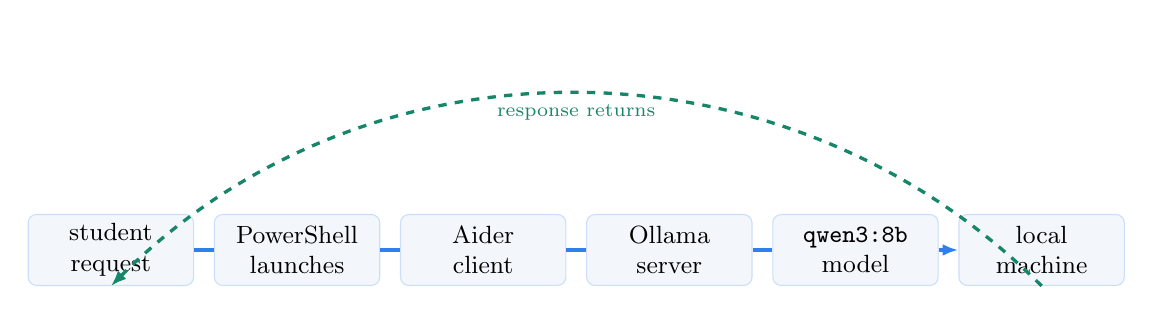
\begin{tikzpicture}[node distance=.25cm,box/.style={draw=blue!25,rounded corners=3pt,fill=mist,minimum width=2.1cm,minimum height=.9cm,align=center,font=\small},arr/.style={-{Latex[length=2mm]},very thick,blue}]\node[box](a){student\\request};\node[box,right=of a](b){PowerShell\\launches};\node[box,right=of b](c){Aider\\client};\node[box,right=of c](d){Ollama\\server};\node[box,right=of d](e){\texttt{qwen3:8b}\\model};\node[box,right=of e](f){local\\machine};\draw[arr](a)--(b)--(c)--(d)--(e)--(f);\draw[arr,dashed,green](f.south)to[bend right=45]node[below,font=\scriptsize]{response returns}(a.south);\end{tikzpicture}\vspace{.65cm}\begin{beamercolorbox}[sep=.7em,wd=.9\linewidth]{block body}\centering One layer working does \textbf{not} prove the next layer works.\end{beamercolorbox}\vfill\ladder\end{frame}
\begin{frame}{Evidence has layers too}\small\renewcommand{\arraystretch}{1.3}\begin{tabular}{p{.22\linewidth}p{.34\linewidth}p{.34\linewidth}}\textbf{Observation}&\textbf{Supports}&\textbf{Does not support}\\\hline\texttt{python --version}&Python command resolves&Your program is correct\\\texttt{ollama list}&Exact model is reported available&The model can answer\\Loopback API check&Local service answered&Aider is integrated\\Direct inference&One model request completed&The answer is correct\\\texttt{git diff}&What text changed&Behavior is correct\\Independent test&Tested behavior passed&Every behavior passed\end{tabular}\vspace{.35cm}\begin{center}\textcolor{gold!80!black}{\textbf{Installed · listed · open · generated are observations, not conclusions.}}\end{center}\end{frame}
\begin{frame}{First: open PowerShell}\begin{columns}[T]\column{.48\linewidth}\begin{enumerate}\item Click Windows \textbf{Start}.\item Type \textbf{PowerShell}.\item Select the provisioned \textbf{PowerShell 7} window.\item Click inside; look for a prompt ending in \texttt{>}.\end{enumerate}\column{.48\linewidth}\begin{beamercolorbox}[sep=.8em,wd=\linewidth]{block body}\texttt{PS C:\textbackslash Users\textbackslash Student>}\par\vspace{.3cm}This is the prompt. It tells you where the command will run.\par\vspace{.3cm}Do not paste a command until you can point to the prompt.\end{beamercolorbox}\end{columns}\vspace{.55cm}\textcolor{blue}{\textbf{FIND THIS YOURSELF:}} “Windows 11 + PowerShell 7: how do I verify which version is actually running? Give the exact command, official Microsoft documentation, and limits.”\end{frame}
\begin{frame}{Verify PowerShell itself}\doit{At the prompt, run: \texttt{\$PSVersionTable.PSVersion}}\whatmeans{PowerShell is the command environment used to navigate folders, launch tools, and repeat checks.}\begin{columns}[T]\column{.48\linewidth}\textbf{DEMAND DOCUMENTATION}\par\scriptsize Find the official Microsoft page for \texttt{PSVersionTable}; check platform relevance.\column{.48\linewidth}\textbf{VERIFY ON YOUR MACHINE}\par\scriptsize Read the version printed by your own terminal. Do not substitute a screenshot.\end{columns}\receipt{Save the command, timestamp, and smallest useful output.}\end{frame}
\begin{frame}{Python: the runtime for our program}\begin{columns}[T]\column{.45\linewidth}\doit{Run: \texttt{python --version}}\whatmeans{Python executes the supplied exercise and its tests.}\column{.48\linewidth}\textbf{What this proves}\begin{itemize}\item The command resolves.\item A runtime reports a version.\end{itemize}\textbf{What it does not prove}\begin{itemize}\item Packages are present.\item Your project or test is correct.\end{itemize}\end{columns}\vfill\textcolor{blue}{\textbf{FIND THIS YOURSELF:}} “Official Python documentation: how do I check the version on Windows, and what does that check leave untested?”\end{frame}
\begin{frame}{Git: the before-and-after witness}\begin{columns}[T]\column{.46\linewidth}\doit{Inside the supplied disposable exercise, run: \texttt{git status} and \texttt{git diff}}\whatmeans{Git exposes the starting state and the exact file change.}\column{.46\linewidth}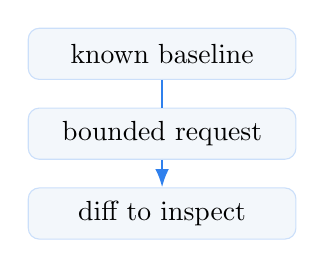
\begin{tikzpicture}[node distance=.35cm,box/.style={draw=blue!25,rounded corners,fill=mist,minimum width=3.4cm,minimum height=.65cm,align=center}]\node[box](a){known baseline};\node[box,below=of a](b){bounded request};\node[box,below=of b](c){diff to inspect};\draw[-{Latex},thick,blue](a)--(b)--(c);\end{tikzpicture}\par\vspace{.3cm}\textbf{Ask:} Which line changed? Which file? Any extras?\end{columns}\vfill\textcolor{blue}{\textbf{DEMAND DOCUMENTATION:}} official Git docs for \texttt{status} and \texttt{diff}.\par\textcolor{green}{\textbf{KEEP THE RECEIPT:}} the diff, not the model's claim.\end{frame}
\begin{frame}{Ollama: a local service on loopback}
\begin{tikzpicture}[node distance=1.15cm,box/.style={draw=blue!25,rounded corners,fill=mist,minimum width=3.5cm,minimum height=.8cm,align=center},arr/.style={-{Latex},very thick}]\node[box](a){Aider\\client};\node[box,right=of a](b){\texttt{127.0.0.1:11434}\\loopback API};\node[box,right=of b](c){Ollama\\local service};\draw[arr,blue](a)--node[above,font=\scriptsize]{request}(b);\draw[arr,green](b)--node[above,font=\scriptsize]{response}(c);\end{tikzpicture}\vspace{.65cm}\doit{Run the approved loopback check supplied by class.}\whatmeans{Loopback names this same computer. A service answering proves reachability—not model inference, privacy of every process, or Aider integration.}\vfill\textcolor{blue}{\textbf{DEMAND DOCUMENTATION:}} Use Ollama's official API documentation; ask what endpoint and response were observed.\end{frame}
\begin{frame}{The exact approved model: \texttt{qwen3:8b}}\begin{columns}[T]\column{.45\linewidth}\doit{Check the exact tag: \texttt{ollama list}}\par\textbf{Then ask:} Did a real request complete?\column{.48\linewidth}\begin{beamercolorbox}[sep=.7em,wd=\linewidth]{block body}\textcolor{gold!80!black}{\textbf{LISTED}}\par model is reported available\vspace{.3cm}\textcolor{green}{\textbf{INFERENCE}}\par model actually answered one request\end{beamercolorbox}\end{columns}\vspace{.45cm}\textcolor{blue}{\textbf{VERIFY ON YOUR MACHINE:}} Send the small approved direct request.\par\receipt{Exact model tag, command, response, exit status.}\end{frame}
\begin{frame}{Aider is the coding client, not the model}\begin{columns}[T]\column{.48\linewidth}\begin{itemize}\item Works from the project folder.\item Gathers bounded file context.\item Communicates with the selected model through Ollama.\item Leaves changes for you to review.\end{itemize}\column{.45\linewidth}\begin{beamercolorbox}[sep=.7em,wd=\linewidth]{block body}\texttt{aider --version}\par\vspace{.25cm}\textbf{Proves:} command reports a version.\par\vspace{.25cm}\textbf{Does not prove:} local Ollama configuration, safe scope, or correct code.\end{beamercolorbox}\end{columns}\vfill\textcolor{blue}{\textbf{BOUNDARY:}} approved profile → \texttt{ollama\_chat/qwen3:8b} → \texttt{http://127.0.0.1:11434}, \texttt{num\_ctx: 8192}. No cloud key or provider detour.\end{frame}
\begin{frame}{The first Aider win: one bounded change}\doit{Start from the supplied disposable Git exercise. Record baseline. Launch the approved local profile. Ask for exactly one narrow change.}\vspace{.5cm}\begin{beamercolorbox}[sep=.8em,wd=\linewidth]{block body}\centering\Large\texttt{baseline → ask → inspect → diff → test}\end{beamercolorbox}\vspace{.55cm}\begin{columns}[T]\column{.48\linewidth}\textbf{A good request}\par\small “Change the supplied function so the expected test passes. Edit only the implementation file. Do not change tests.”\column{.48\linewidth}\textbf{A bad request}\par\small “Fix everything, improve the project, and make it production-ready.”\end{columns}\vfill\textcolor{gold!80!black}{Scope is a safety feature.}\end{frame}
\begin{frame}{Inspect the diff before you trust it}\begin{columns}[T]\column{.47\linewidth}\doit{Exit Aider, then run the approved \texttt{Diff} command.}\column{.47\linewidth}\begin{beamercolorbox}[sep=.7em,wd=\linewidth]{block body}\textbf{Look for:}\begin{itemize}\item intended file only;\item intended line(s) only;\item no secret, test, or unrelated edits;\item a change you can explain.\end{itemize}\end{beamercolorbox}\end{columns}\vfill\begin{center}\textcolor{gold!80!black}{\Large\textbf{“Aider changed it” is not “the change is correct.”}}\end{center}\end{frame}
\begin{frame}{Independent test: a different claim}\begin{columns}[T]\column{.47\linewidth}\doit{Run the supplied independent final test.}\column{.47\linewidth}\whatmeans{A test reruns a defined behavior without trusting the model's narration.}\begin{beamercolorbox}[sep=.6em,wd=\linewidth]{block body}\textbf{Passing supports:} the behavior this test checks.\par\vspace{.2cm}\textbf{Not proof of:} every input, every file, or every possible property.\end{beamercolorbox}\end{columns}\vfill\receipt{Preserve exit status and smallest useful test output.}\end{frame}
\begin{frame}{Three tiny wins: repeat the loop}\centering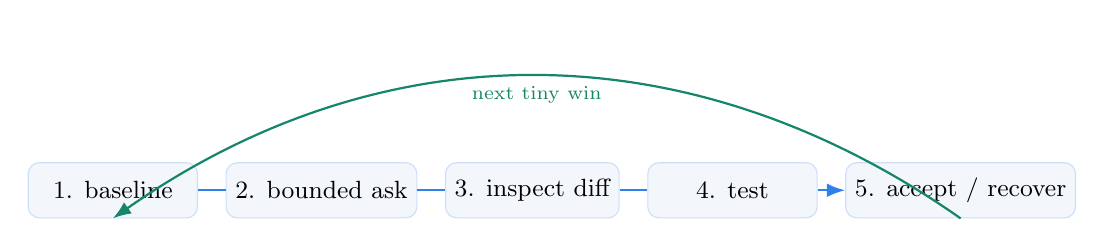
\begin{tikzpicture}[node distance=.35cm,stage/.style={draw=blue!25,rounded corners,fill=mist,minimum width=2.15cm,minimum height=.7cm,align=center,font=\small}]\node[stage](a){1. baseline};\node[stage,right=of a](b){2. bounded ask};\node[stage,right=of b](c){3. inspect diff};\node[stage,right=of c](d){4. test};\node[stage,right=of d](e){5. accept / recover};\draw[-{Latex},thick,blue](a)--(b)--(c)--(d)--(e);\draw[-{Latex},thick,green](e.south)to[bend right=35]node[below,font=\scriptsize]{next tiny win}(a.south);\end{tikzpicture}\vspace{.7cm}\begin{columns}[T]\column{.3\linewidth}\textbf{Win 1}\par visible edit\column{.3\linewidth}\textbf{Win 2}\par test-backed repair\column{.3\linewidth}\textbf{Win 3}\par harmless student-directed change\end{columns}\vfill\textcolor{blue}{Each loop earns a little more independence.}\end{frame}
\begin{frame}{Recovery is part of the workflow}\begin{columns}[T]\column{.48\linewidth}\begin{beamercolorbox}[sep=.8em,wd=\linewidth]{block body}\centering\Huge\textbf{“NOT READY”}\par\vspace{.3cm}\normalsize is useful evidence.\end{beamercolorbox}\vspace{.45cm}\textbf{Stop at the first failed check.}\par Record the claim, command, exit status, smallest output, and diagnostic code.\column{.46\linewidth}\textbf{One bounded retry}\begin{enumerate}\item Confirm the supplied folder.\item Run the same documented check once.\item Escalate if it still fails.\end{enumerate}\textbf{Do not:} switch models, scan ports, add credentials, download, elevate, or repeatedly repair services.\end{columns}\vfill\textcolor{green}{Recitation is the recovery seam—not a reason to improvise infrastructure.}\end{frame}
\begin{frame}{Prompt structure: from answer to evidence}\begin{columns}[T]\column{.3\linewidth}\begin{beamercolorbox}[sep=.5em,wd=\linewidth]{block body}\textcolor{gold!80!black}{\textbf{WEAK}}\par “How do I check PowerShell?”\end{beamercolorbox}\column{.3\linewidth}\begin{beamercolorbox}[sep=.5em,wd=\linewidth]{block body}\textbf{BETTER}\par “Windows 11 + PowerShell 7: give exact command and expected output.”\end{beamercolorbox}\column{.3\linewidth}\begin{beamercolorbox}[sep=.5em,wd=\linewidth]{block body}\textbf{VERIFICATION-ORIENTED}\par “Cite Microsoft docs; say what it proves and does not prove; give an independent check.”\end{beamercolorbox}\end{columns}\vspace{.7cm}\begin{center}\Large\textcolor{gold!80!black}{\textbf{Do not stop at the answer. Ask how to verify it.}}\end{center}\vfill\textcolor{blue}{\textbf{FIND THIS YOURSELF:}} build the question with platform, version, action, observation, primary source, and limits.\end{frame}
\begin{frame}{Learning to fish: the scaffold fades}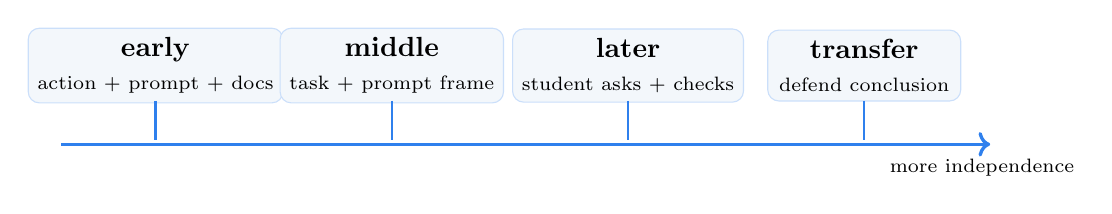
\begin{tikzpicture}[x=1cm,y=1cm]\draw[->,very thick,blue](.5,0)--(12.3,0);\node[font=\scriptsize,anchor=west]at(10.9,-.3){more independence};\foreach \x/\t/\d in {1.7/{early}/{action + prompt + docs},4.7/{middle}/{task + prompt frame},7.7/{later}/{student asks + checks},10.7/{transfer}/{defend conclusion}}{\node[draw=blue!25,rounded corners,fill=mist,align=center,minimum width=2.45cm,minimum height=.85cm]at(\x,1){\textbf{\t}\\\scriptsize\d};\draw[blue,thick](\x,.55)--(\x,.05);}\end{tikzpicture}\vspace{.5cm}\begin{columns}[T]\column{.48\linewidth}\textbf{Your job changes:} from following a recipe to choosing a defensible check.\column{.46\linewidth}\textbf{The habit stays:} claim → observation → limit → conclusion.\end{columns}\vfill\ladder\end{frame}
\begin{frame}{Work First: the bridge}\centering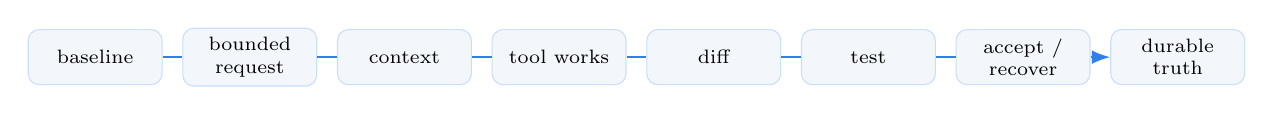
\begin{tikzpicture}[node distance=.25cm,stage/.style={draw=blue!25,rounded corners,fill=mist,minimum width=1.7cm,minimum height=.7cm,align=center,font=\scriptsize}]\node[stage](a){baseline};\node[stage,right=of a](b){bounded\\request};\node[stage,right=of b](c){context};\node[stage,right=of c](d){tool works};\node[stage,right=of d](e){diff};\node[stage,right=of e](f){test};\node[stage,right=of f](g){accept /\\recover};\node[stage,right=of g](h){durable\\truth};\draw[-{Latex},thick,blue](a)--(b)--(c)--(d)--(e)--(f)--(g)--(h);\end{tikzpicture}\vspace{.7cm}\begin{beamercolorbox}[sep=.7em,wd=.9\linewidth]{block body}\centering Work First means knowing the starting state, bounding the work, inspecting evidence, testing independently, and preserving what remains true.\end{beamercolorbox}\vfill\textcolor{blue}{This week is the small, teachable version of a professional loop.}\end{frame}
\begin{frame}{Show that it works: the Week 2 receipt}\begin{columns}[T]\column{.46\linewidth}\textbf{By the end, demonstrate:}\begin{itemize}\item PowerShell and foundation checks;\item direct Ollama success with exact \texttt{qwen3:8b};\item one bounded Aider change;\item inspected \texttt{git diff};\item independent test result;\item one sentence explaining the loop.\end{itemize}\column{.46\linewidth}\begin{beamercolorbox}[sep=.7em,wd=\linewidth]{block body}\textbf{Receipt}\par\scriptsize Claim · command · exit status · smallest output · conclusion · limit\par\vspace{.3cm}\textbf{If not ready}\par\scriptsize Preserve failure evidence and use Recitation/support.\end{beamercolorbox}\end{columns}\vfill\begin{center}\Large\textcolor{green}{\textbf{A small receipt beats a confident story.}}\end{center}\end{frame}
\begin{frame}[plain]\begin{tikzpicture}[remember picture,overlay]\fill[navy](current page.south west)rectangle(current page.north east);\fill[green](current page.south west)rectangle([xshift=5.2cm]current page.south west);\end{tikzpicture}\vspace{2cm}\color{white}\Huge\textbf{Your turn}\par\vspace{.6cm}\Large\color{white!85}Ask narrowly. Inspect honestly. Test independently. Keep the receipt.\par\vspace{1.2cm}\color{gold}\Large\textbf{What does this prove?}\end{frame}
\end{document}
